\documentclass[10pt,a4paper]{article}
\usepackage[utf8]{inputenc}
\usepackage{amsmath}
\usepackage{amsfonts}
\usepackage{amssymb}
\usepackage{graphicx}
\usepackage{float}
\usepackage[hidelinks]{hyperref}
\usepackage[left=1in,right=1in,top=1in,bottom=1in]{geometry}

\title{Pipeline control protocol for the Otter MCU}
\author{Trevor McKay}
\date{Summer 2020}

\graphicspath{{./figures/}}

\begin{document}

\begin{center}
    \Large\textbf{RISC-V UART Debugger\\Implementation}

    \medskip
    \small{for CPE-233}
\end{center}

\tableofcontents
\newpage

\section{Introduction}
The debugger client and modules allow for instant programming of your Otter without Vivado and
powerful debugging features such as pausing execution, breakpoints, register access,
and memory access.

To use the debugger, the first step is to get a hold of the modules and the debugging client.
Everything is included in a GitHub repository. Clone the repository to download all the necessary
files:

\begin{verbatim}
git clone git@github.com:trmckay/universal-otter-debugger.git
\end{verbatim}

The debugger currently only supports Linux and macOS, though it can be used in Windows via WSL.

\section{Integrating the debugger with your Otter}

\subsection{Adding the files}
From the repository, include all the SystemVerilog files in \emph{uart-db/module/design} as well as
\emph{otter-adapter/multicycle/db\_adapter.sv} in your Vivado project. Or, add them from wherever
you downloaded them. You will add a total of seven files.

\subsection{Adding UART connections to the Otter}

In your wrapper, add a one bit output \emph{stx} and a one bit input \emph{srx}.

\medskip
\noindent\underline{File: \emph{otter\_wrapper.sv}}
\begin{verbatim}
    module OTTER_Wrapper (
        // other I/O...
        input srx,
        output stx
    );
\end{verbatim}

\noindent Do the same in the MCU.

\medskip
\noindent\underline{File: \emph{otter\_mcu.sv}}
\begin{verbatim}
    module OTTER_MCU (
        // other I/O...
        input srx,
        output stx
    );
\end{verbatim}

\noindent Where the MCU is instantiated in the wrapper, connect the new signals.

\medskip
\noindent\underline{File: \emph{otter\_wrapper.sv}}
\begin{verbatim}
    OTTER_MCU MCU(
        // other I/O...
        .srx(srx),
        .stx(stx)
    );
\end{verbatim}

You will need to modify the constraints to connect \emph{srx} and \emph{stx} to the micro-USB port
on the Basys3. Paste the following into your constraints:

\begin{verbatim}
    ##USB-RS232 Interface
    set_property PACKAGE_PIN B18 [get_ports srx]
        set_property IOSTANDARD LVCMOS33 [get_ports srx]
    set_property PACKAGE_PIN A18 [get_ports stx]
        set_property IOSTANDARD LVCMOS33 [get_ports stx]
\end{verbatim}

\subsection{Modifying the FSM}
The FSM requires some very small modifications to accomodate the debugger. It needs the ability to
pause as well as a new output for the present state.

Add a one bit input to your MCU called \emph{pause} and a two bit output for the state.

\begin{verbatim}
    module cu_fsm (
        // other I/O...
        input pause,
        output [1:0] state
    );
\end{verbatim}

The state output can simply be assigned to the present state variable.

\begin{verbatim}
    assign state = ps;
\end{verbatim}

The signal \emph{pause} should prevent your FSM from changing states while high. This can be done
by adding a conditional around the state transition.

\medskip
\noindent\textbf{Before}:
\begin{verbatim}
    always_ff @(posedge clk)
        ps <= ns;
\end{verbatim}

\noindent\textbf{After}:
\begin{verbatim}
    always_ff @(posedge clk) begin
        if (!pause)
            ps <= ns;
    end
\end{verbatim}

\newpage
\subsection{Instantiation and variable declaration}
Add the module to your MCU and connect the relevent signals. Here is a template instantiation
with the output variables declared.

\begin{verbatim}
    wire db_active, db_fsm_pause, db_mem_rd, db_mem_wr, db_rf_rd, db_rf_wr, db_reset;
    wire [1:0] db_mem_size;
    wire [31:0] db_mem_addr, db_d_wr;
    wire [4:0] db_rf_addr;

    db_adapter_mc debugger(
        .srx(srx),                    // serial input
        .stx(stx),                    // serial output
        .clk(),                       // 50 MHz clock
        .pc(),                        // program count
        .mcu_ps(),                    // present state of FSMi
        .opcode(),                    // opcode of current instruction
        .mem_d_out(),                 // data out 2 from memory
        .rf_d_out(),                  // rs1 output from register file
        .db_active(db_active),        // debugger is active
        .db_fsm_pause(db_fsm_pause),  // fsm should remain paused
        .db_mem_addr(db_mem_addr),    // address for memory access
        .db_mem_size(db_mem_size),    // size of memory access
        .db_mem_wr(db_mem_wr),        // write enable for memory
        .db_mem_rd(db_mem_rd),        // read enable for memory
        .db_rf_addr(db_rf_addr),      // address for register access
        .db_rf_wr(db_rf_wr),          // write enable for register file
        .db_rf_rd(db_rf_rd),          // read enable for register file
        .db_d_wr(db_d_wr),            // write data for register file and memory
        .db_reset(db_reset)           // reset PC and FSM
    );
\end{verbatim}

\newpage
\subsection{Connections in the MCU}
Below is a diagram of the necessary connections in the Otter.

\bigskip
\begin{figure}[htpb]
    \centering
    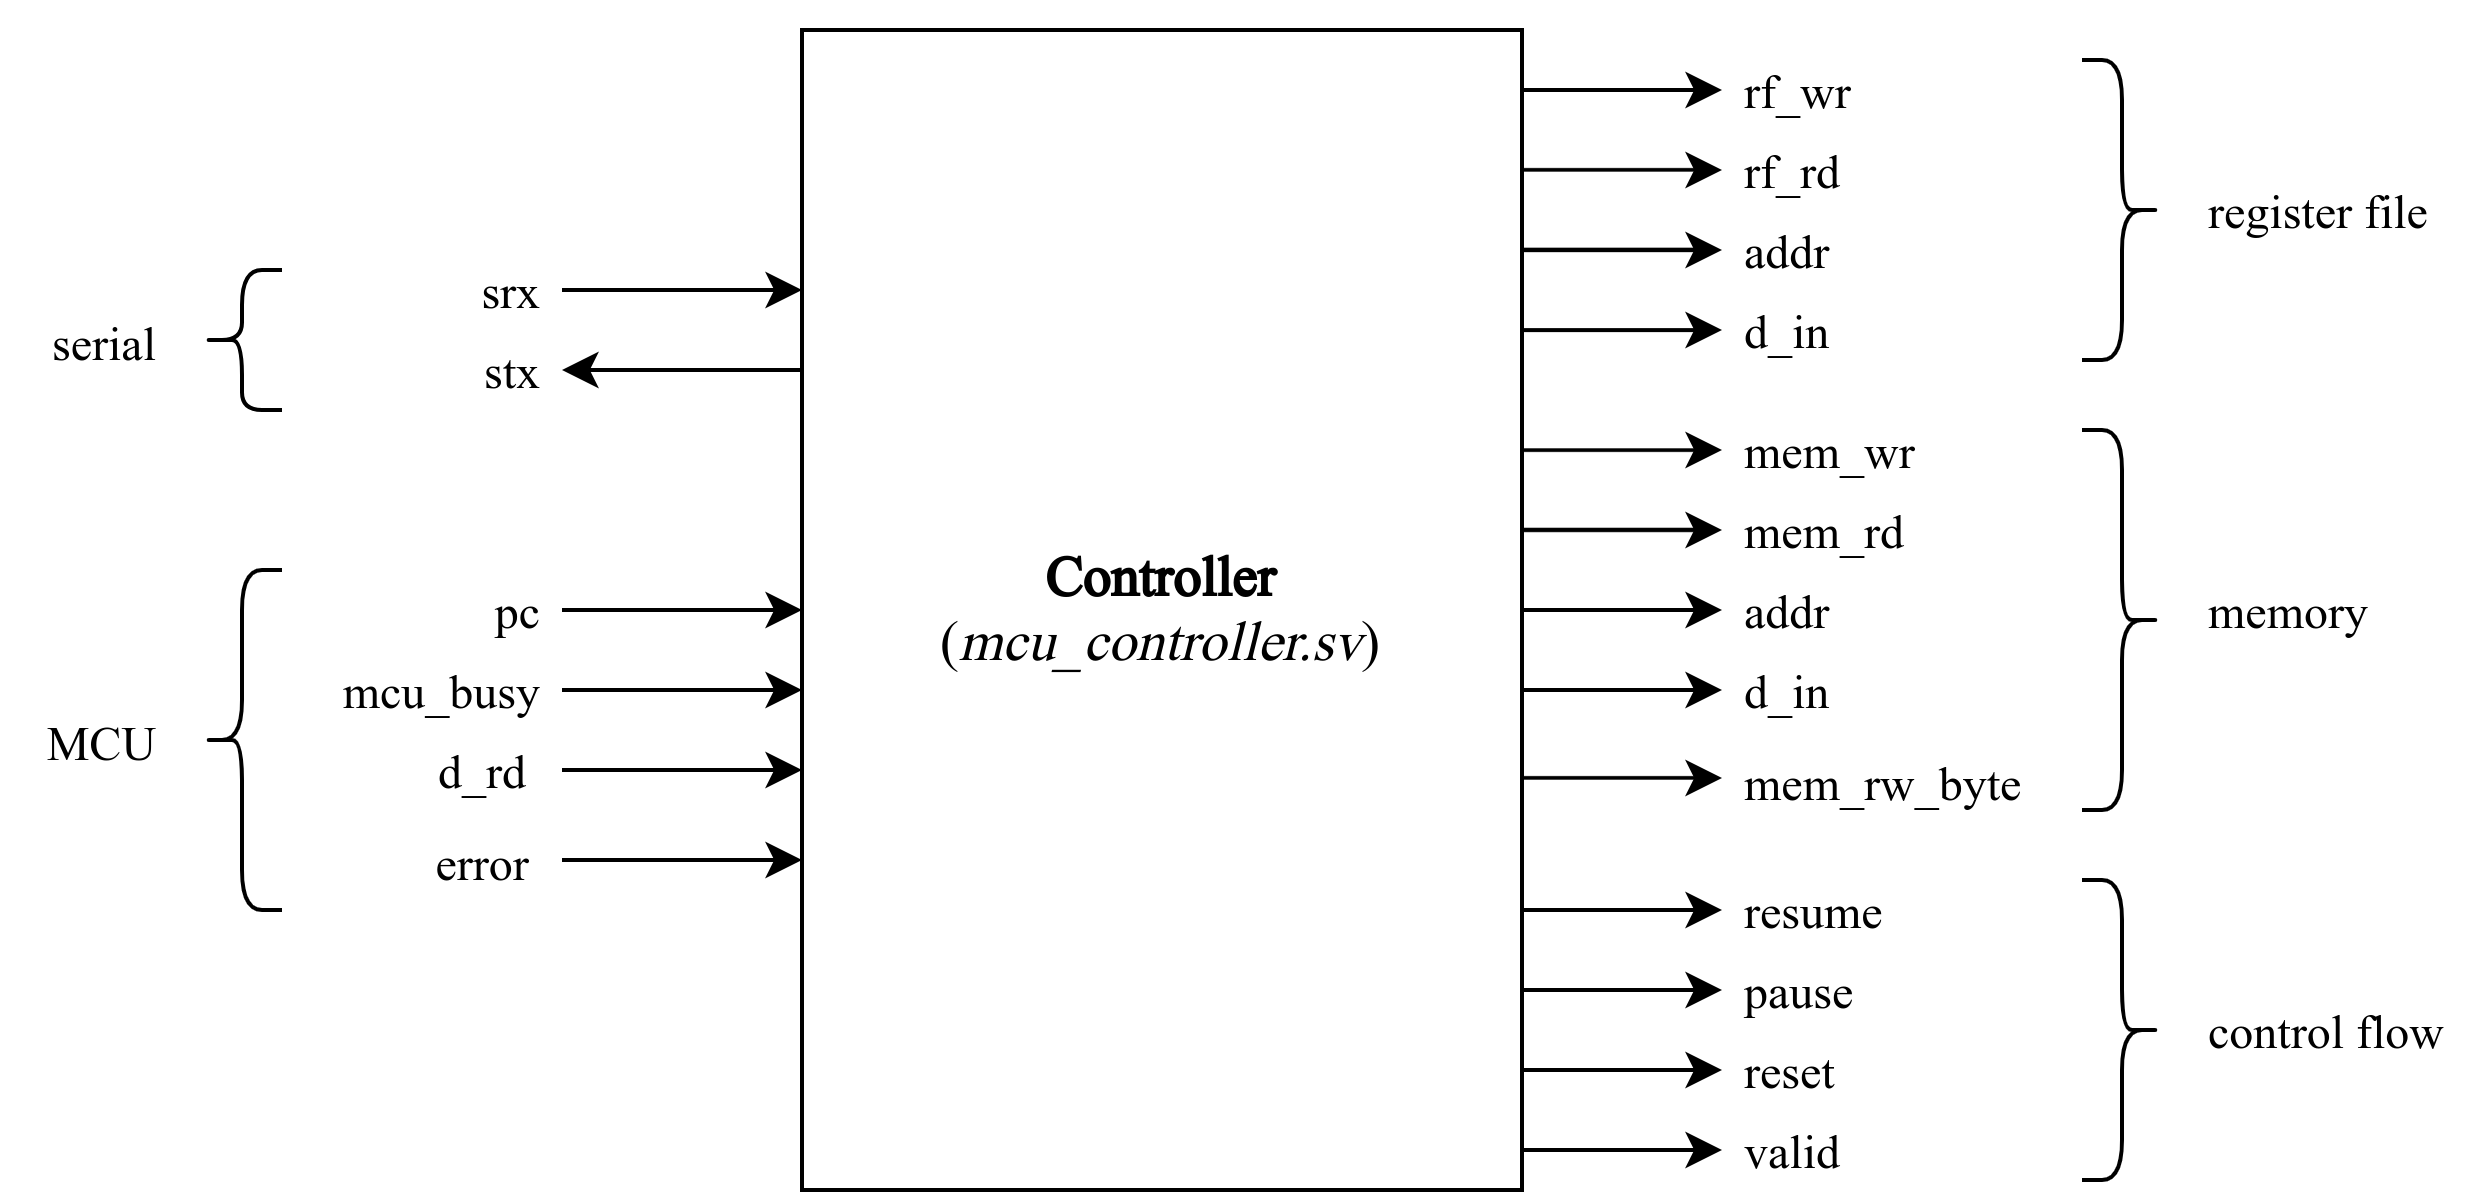
\includegraphics[width=\linewidth]{blackbox.png}
\end{figure}

\newpage
Alternatively, the modifications are described textually below. Only the modified connections
are listed and variable names may vary.

\medskip

\textbf{Program counter}
\begin{verbatim}
    program_counter PC(
        .load(pc_write && !db_active),
        .reset(reset || db_reset)
    );
\end{verbatim}

\textbf{Register file}
\begin{verbatim}
    program_counter PC(
        .read_addr1((db_rf_rd) ? db_rf_addr : ir[19:15]),
        .write_addr((db_rf_rd) ? db_rf_addr : ir[11:7]),
        .write_data((db_rf_wr) ? db_d_wr : rf_data_in),
        .write_enable(rf_wr || db_rf_wr)
    );
\end{verbatim}

\textbf{Memory}
\begin{verbatim}
    OTTER_mem_byte #(14) memory (
        .MEM_ADDR2((db_active) ? db_mem_addr : alu_result),
        .MEM_DIN2((db_active) ? db_d_wr : rs2),
        .MEM_WRITE2(memWrite || db_mem_wr),
        .MEM_READ1(memRead1 && !db_active),
        .MEM_READ2(memRead2 || db_mem_rd),
        .MEM_SIZE((db_active) ? db_mem_size : ir[13:12]),
    );
\end{verbatim}

\textbf{FSM}
\begin{verbatim}
    otter_fsm FSM(
        .reset(mcu_reset || db_reset),
        .state(mcu_ps),
        .pause(db_fsm_pause)
    );
\end{verbatim}

\section{Debugging client}
\subsection{Installation}
Using and installing the debug client is very simple. To clone the source code, build, and install,
run the install script in the \emph{uart-db} folder in the repository. Follow the instructions in
your terminal, and installation should be easy. Be sure to scan the output of the installer for
any warnings.

\subsection{Usage}
When installation is complete, launch the debugger with the command \emph{uart-db}. If you agree to
autodetect, it will automatically connect to the Otter. If you already know the location of your
serial port, you can launch the client with \emph{uart-db [device path]}. Once in the debugging shell,
enter \emph{h} or \emph{help} to output the help message.

\vspace*{\fill}
\begin{center}
    \noindent Contact Trevor McKay with questions.\\
    \href{mailto:trmckay@calpoly.edu}{trmckay@calpoly.edu}
\end{center}

\end{document}
